\section{Chemical process}\label{se:chemical_process}

\fxnote{Illustrering af fig 1,1 hvitved og dertil beskrivelse af den, for at give et overblik over kloakker og dens processer}

\subsection{Chemical reactions in a sewer}\label{subse:chemical_reactions_in_a_sewer}
A wastewater treatment plant receive not only what is discharged into the sewer from the industry and households but also the chemical and microbial reactions that occurs in a sewer. Within these sewers different redox reactions occurs under different conditions, these condition are aerobic, anoxic or anaerobic.    %These processes can affect other parts of the system e.g. some reactions may lead to malodorous substances that will reach the urban atmosphere. 



\begin{figure}[H]
\centering
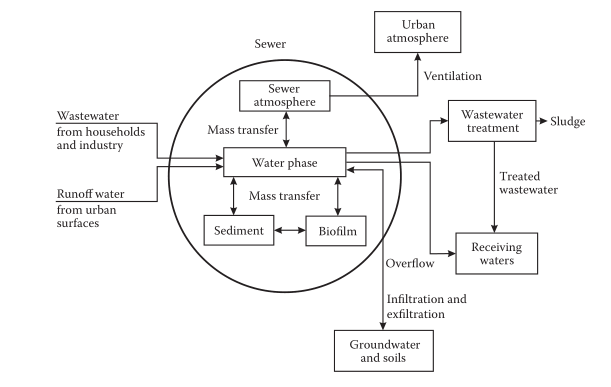
\includegraphics[width=1\textwidth]{report/introduction/pictures/sewer_overview_of_the_different_parts.png}
\caption{Illustrates how the wastewater flows from the industry and households to the treatment plant. \fxnote{Ny tegning}}
\label{fig:sewer_overview_of_the_different_parts}
\end{figure}


\subsection{Wastewater treatment plant}\label{subse:Wastewater treatment plant}

